\documentclass[5pt]{article}
\usepackage{graphicx}
\usepackage{booktabs}

\begin{document}

\title{Assignment 2}
\author{Mukul Sati [msati3@gatech.edu]}
\maketitle

\section{Random forests trained with bagging}
I carried out two iterations of the following experiment: I trained multiple
random forests, with varying number of decision trees (I used the
implementation in sklearn). I let the decision trees grow unconstrained during
the first iteration, and limited their depth to 5 levels during the second. I
create bagged sets of size 1/3 of the training set for both the iterations.

\subsection{Wine dataset}
For the wine dataset, I selected a random subset of size 75\% of the original
data for training. I did not ensure that the samples in the training set are
equally distributed for each label. While this is sub-optimal as mentioned by
the instructor on Piazza, I think the split of {33\%, 40\%, 27\%} amongst the
  classes is not substantial to adversely affect the results.

The plots for the errors for the two iterations are shown in
Fig.~\ref{fig:errorsWine}.

\begin{figure}
  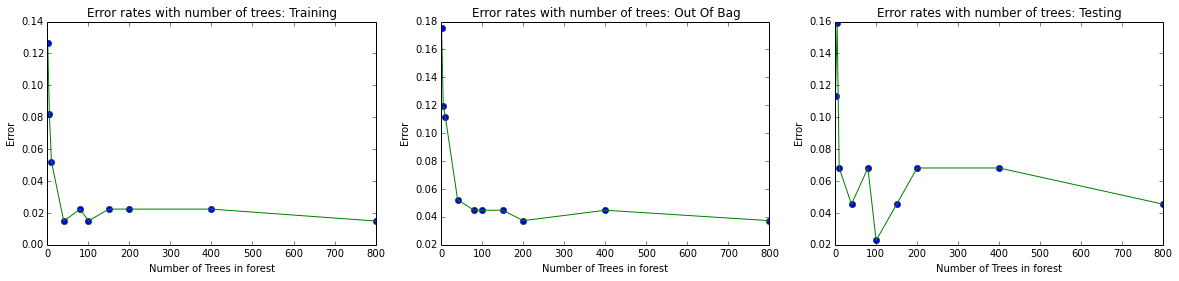
\includegraphics[width=\textwidth]{images/baggingDepthInfiniteWine.png}
  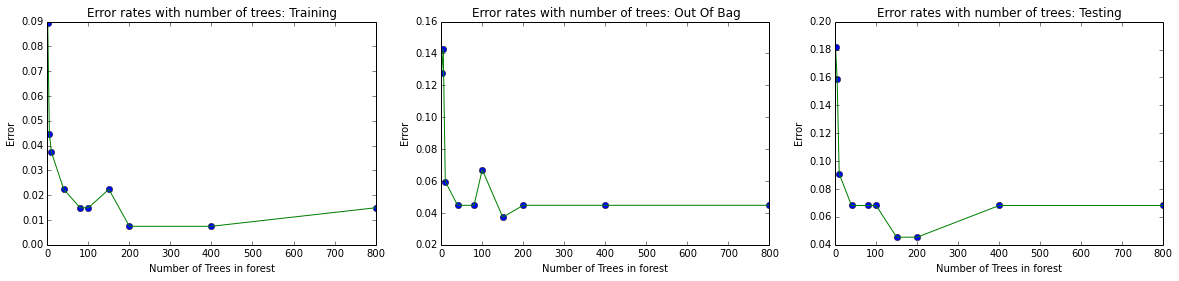
\includegraphics[width=\textwidth]{images/baggingDepthLimitedWine.png}
\label{fig:errorsWine}
\caption{The errors on the (a) Training, (b) Out of bag and (c) Testing data
  when using unconstrained depth binary trees (top) and when using binary trees
  that are only allowed to grow to depth 5 (bottom) for the wine dataset}
\end{figure}

The confusion matrix for the wine-data for a Random Forest with 100
depth-not-limited trees and one with 150 depth-limited (to 5 levels) trees
respectively is shown
in Table~\ref{tab:confusionWine}

\begin{table}
\centering
\begin{tabular}{cccc}
\toprule
Label & 1 & 2 & 3\\
\midrule
  1 & 10 & 1 & 0\\
  2 & 0 & 21 & 0\\
  3 & 0 & 0 & 12\\
\bottomrule
\end{tabular}
\quad
\begin{tabular}{cccc}
\toprule
Label & 1 & 2 & 3 \\
\midrule
  1 & 10 & 1 & 0 \\
  2 & 1 & 20 & 0 \\
  3 & 0 & 0 & 12 \\
\bottomrule
\end{tabular}
\caption{The confusion matrix for a Random Forest with 100 depth-not-limited
  trees (left). The confusion for a Random Forest with 150 depth-limited to 5
trees (right). These results are for the wine-dataset.}
\label{tab:confusionWine}
\end{table}

\subsection{MNIST dataset}
For MNIST, I used PCA to reduce dimensionality, retaining enough principal
component vectors that explain 80\% of the variance in the data. I feel this
gives me a good balance between a performant algorithm and execution time. The
plots for the errors for the two iterations are shown in
Fig.~\ref{fig:errorsMNIST}.

\begin{figure}
  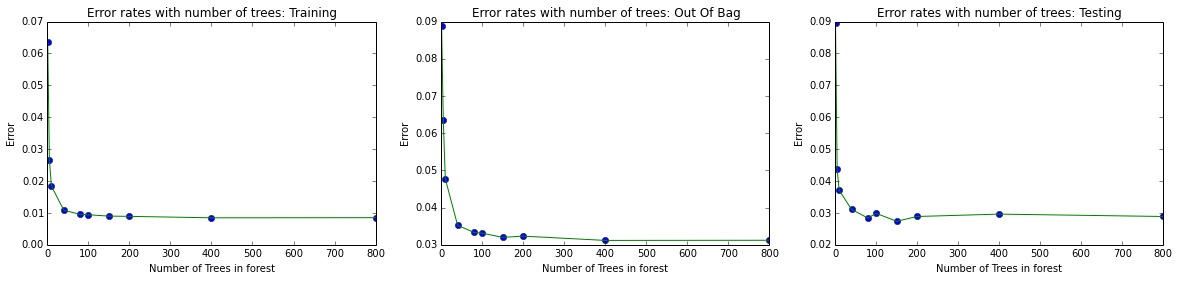
\includegraphics[width=\textwidth]{images/baggingDepthInfiniteMNIST.png}
  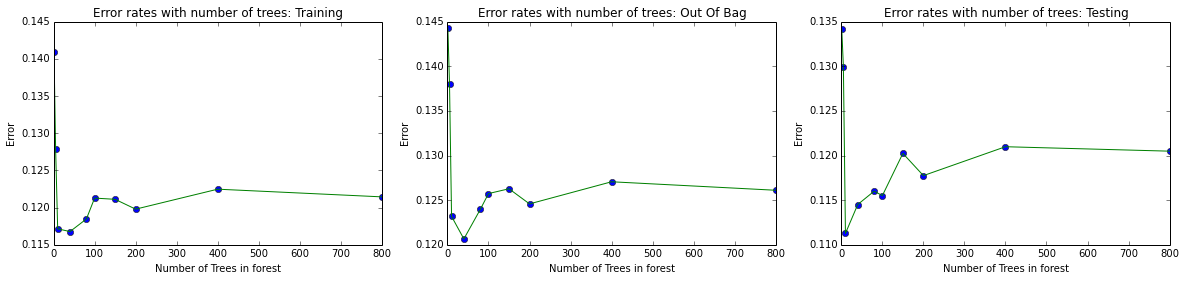
\includegraphics[width=\textwidth]{images/baggingDepthLimitedMNIST.png}
\label{fig:errorsMNIST}
\caption{The errors on the (a) Training, (b) Out of bag and (c) Testing data
  when using unconstrained depth binary trees (top) and when using binary trees
  that are only allowed to grow to depth 5 (bottom) for the MNIST dataset}
\end{figure}

The confusion matrix for the MNIST dataset for a Random Forest with 100
depth-not-limited trees and one with 150 depth-limited (to 5 levels) trees
respectively is shown
in Table~\ref{tab:confusionMNIST}
\begin{table}
\centering
\begin{tabular}{ccccc}
\toprule
Digit & 0 & 1 & 3 & 5 \\
\midrule
0 & 964 & 0 & 7 & 9\\
1 & 0 & 1126 & 5 & 4\\
3 & 4 & 4 & 972 & 30\\
5 & 18 & 1 & 28 & 845\\
\bottomrule
\end{tabular}
\quad
\begin{tabular}{ccccc}
\toprule
Digit & 0 & 1 & 3 & 5\\
\midrule
0 & 852 & 0 & 26 & 102\\
1 & 0  & 1092 &  14 & 29\\
3 & 13 & 8 & 847 & 142\\
4 & 42 & 4 & 80 & 766\\
\bottomrule
\end{tabular}
\caption{The confusion matrix for a Random Forest with 150 depth-not-limited
  trees (left). The confusion for a Random Forest with 40 depth-limited to 5
trees (right). These results are for the MNIST dataset.}
\label{tab:confusionMNIST}
\end{table}

\subsection{Discussion}
My observations are in line with~\cite{breiman2001random}. The training error
soon plateaus in both the cases (depth limited and unconstrained decision
trees). However, the out of bag error still decreases for a while post this.
This may be explained in terms of margin function (the difference between the
number of correct class predictions, and the maximum over the number of incorrect
predictions for a given incorrect class), is driven to its limiting value of the
probabilities of the two classes under consideration over the feature space.
Thus, the generalization error may still decrease even after the training error
plateaus, due to improving probability margins between confusable classes. This
effect is observed in the training errors, where they decrease (see
particularly, Fig.~\ref{fig:errorsMNIST}) with increasing number of trees, due
to improving generalization.

\section{Boosting}
I have (tried to) implemented the AdaBoost.M2 algorithm as described
in~\cite{freund1996experiments}. Using both a decision stump, and a decision
tree limited to grow to depth 10 as the weak learners, I train boosted
ensembles
with a varying number of weak learners in them.

\subsection{MNIST dataset}
For MNIST, similar to bagging, I used PCA to reduce dimensionality, retaining
enough principal component vectors that explain 80\% of the variance in the
data. I feel this gives me a good balance between a performant algorithm and
execution time.  The plots for the errors for the two iterations are shown in
Fig.~\ref{fig:errorsMNISTBoosting}.

\begin{figure}
  \includegraphics[width=\textwidth]{images/boostingDepthInfiniteMNIST.png}
  \includegraphics[width=\textwidth]{images/boostingDepthLimitedMNIST.png}
\label{fig:errorsMNISTBoosting}
\caption{The errors on the (a) Training and (b) Testing data when
  using boosted decision stumps (top) and when using boosted decision trees
that are only allowed to grow to depth 10 (bottom) for the MNIST dataset}
\end{figure}

The confusion matrix for the MNIST dataset for an ensemble of 100 boosted
decision tree stumps and one with 150 depth-limited (to 10 levels)
decision trees respectively is shown in Table~\ref{tab:confusionMNISTBoost}
\begin{table}
\centering
\begin{tabular}{ccccc}
\toprule
Digit & 0 & 1 & 3 & 5 \\
\midrule
0 & 964 & 0 & 7 & 9\\
1 & 0 & 1126 & 5 & 4\\
3 & 4 & 4 & 972 & 30\\
5 & 18 & 1 & 28 & 845\\
\bottomrule
\end{tabular}
\quad
\begin{tabular}{ccccc}
\toprule
Digit & 0 & 1 & 3 & 5\\
\midrule
0 & 852 & 0 & 26 & 102\\
1 & 0  & 1092 &  14 & 29\\
3 & 13 & 8 & 847 & 142\\
4 & 42 & 4 & 80 & 766\\
\bottomrule
\end{tabular}
\caption{The confusion matrix for a boosted ensemble of decision tree stumps
  trained over 100 iterations (left). The confusion for a boosted ensemble of
  150 depth-limited to 10 decision trees (right). These results are for the MNIST
dataset.}
\label{tab:confusionMNISTBoost}
\end{table}

\subsection{Office Dataset}
**Not worked on**

\subsection{Discussion}
Boosting performance using decision tree stumps is poor for the 4 class
problem, as only two possible classes can be identified by each decision tree.
However, this performance is better than the weak learner we started with. As
expected, the performance when using decision trees with a maximum depth of 10
is much improved due to it being a stronger learner. In~\cite{freund1999short},
in an analogous manner to~\cite{breiman2001random}, the authors attempt to
explain the paradox of not-overfitting with increasing number of learners in
the ensemble --- contrary to what would be expected using VC-dimension based
arguments --- with margin theory, even drawing some parallels with SVMs. I don't
observe the same results on my experiments, and I'd hazard a guess that this is
due to a bug in my code.

\medskip
\bibliographystyle{unsrt}
\bibliography{references}
\end{document}
